\documentclass[a4paper]{article}

\def\npart {UF PHA 6125}
\def\nterm {Lesson 1A/1B}
\def\nyear {2026}
\def\nlecturer {Lalonde and Cristofoletti; FDA/ICH updates}
\def\ncourse {Drug Development and Fundamental PK/PD}
\def\ncoursehead {Lesson 1 PK/PD}
\def\nauthor {NanFangHong}

\RequirePackage{etex}
\makeatletter
\ifx \npart \undefined
  \def\npart{PK/PD Notes}
\fi
\ifx \nterm \undefined
  \def\nterm{Reading notes}
\fi
\ifx \nyear \undefined
  \def\nyear{\the\year}
\fi
\ifx \nlecturer \undefined
  \def\nlecturer{the source literature}
\fi
\ifx \nauthor \undefined
  \def\nauthor{NanFangHong}
\fi
\ifx \ncourse \undefined
  \def\ncourse{Pharmacology Reading Note}
\fi
\ifx \ncoursehead \undefined
  \def\ncoursehead{\ncourse}
\fi

\author{Based on \nlecturer \\\small Notes taken by \nauthor}
\date{\nterm\ \nyear}
\title{\npart\ --- \ncourse}

\usepackage{amsfonts}
\usepackage{amsmath}
\usepackage{amssymb}
\usepackage{amsthm}
\usepackage{booktabs}
\usepackage{caption}
\usepackage{enumitem}
\usepackage{fancyhdr}
\usepackage{fontspec}
\usepackage{graphicx}
\usepackage{iftex}
\usepackage{mathtools}
\usepackage{microtype}
\usepackage{siunitx}
\usepackage{tabularx}
\usepackage{tikz}
\usepackage{xcolor}
\usepackage{xurl}
\usepackage{xeCJK}

\IfFontExistsTF{Latin Modern Roman}{
  \setmainfont[Ligatures=NoCommon]{Latin Modern Roman}
}{}

\IfFontExistsTF{Noto Serif CJK SC}{
  \setCJKmainfont{Noto Serif CJK SC}
}{
  \IfFontExistsTF{Songti SC}{
    \setCJKmainfont{Songti SC}
  }{
    \IfFontExistsTF{PingFang SC}{
      \setCJKmainfont{PingFang SC}
    }{}
  }
}

\usepackage[hidelinks,unicode,breaklinks=true]{hyperref}
\hypersetup{
  pdfauthor={\nauthor},
  pdfsubject={\npart\ - \ncourse},
  pdftitle={\npart\ - \ncourse},
  pdfkeywords={PK PD pharmacology reading notes \ncourse}
}

\pagestyle{fancyplain}
\lhead{\emph{\nouppercase{\leftmark}}}
\rhead{
  \ifnum\thepage=1
  \else
    \npart\ \ncoursehead
  \fi}

\theoremstyle{definition}
\newtheorem*{aim}{Aim}
\newtheorem*{assumption}{Assumption}
\newtheorem*{defi}{Definition}
\newtheorem*{eg}{Example}
\newtheorem*{notation}{Notation}
\newtheorem*{question}{Question}
\newtheorem*{remark}{Remark}
\newtheorem*{warning}{Warning}

\theoremstyle{plain}
\newtheorem{nthm}{Theorem}[section]
\newtheorem{nprop}[nthm]{Proposition}

\renewcommand{\labelitemi}{--}
\renewcommand{\labelitemii}{$\circ$}
\renewcommand{\labelenumi}{(\roman{*})}

\let\stdsection\section
\renewcommand\section{\newpage\stdsection}

\newcommand{\dd}{\mathop{}\!\mathrm{d}}
\newcommand{\Emax}{E_{\max}}
\newcommand{\pksym}[1]{\ifmmode\text{\textit{#1}}\else\textit{#1}\fi}
\newcommand{\pklab}[1]{\mathrm{#1}}
\newcommand{\ECfifty}{\pksym{EC}_{50}}
\newcommand{\term}[1]{\emph{#1}}
\makeatother

\usetikzlibrary{arrows.meta,positioning,calc,shapes.geometric,decorations.pathreplacing}
\emergencystretch=4em
\captionsetup{width=0.9\textwidth, justification=raggedright, singlelinecheck=false}
\lhead{\emph{\npart}}
\rhead{\ncoursehead}

\renewcommand{\Emax}{\ensuremath{E_{\max}}}
\renewcommand{\ECfifty}{\ensuremath{\pksym{EC}_{50}}}
\DeclareMathOperator*{\argmin}{arg\,min}
\newcommand{\Prob}{\mathbb{P}}
\newcommand{\Ex}{\mathbb{E}}
\newcommand{\Normal}{\mathcal{N}}
\newcommand{\data}{\mathcal{D}}
\newcommand{\given}{\,|\,}
\newcommand{\rv}[1]{\mathsf{#1}}
\newcommand{\CL}{\ensuremath{\pksym{CL}}}
\newcommand{\Vd}{\ensuremath{\pksym{V}_d}}
\newcommand{\AUC}{\ensuremath{\pksym{AUC}}}
\newcommand{\AUMC}{\ensuremath{\pksym{AUMC}}}
\newcommand{\Cmax}{\ensuremath{C_{\pklab{max}}}}
\newcommand{\Tmax}{\ensuremath{T_{\pklab{max}}}}
\newcommand{\ka}{\ensuremath{k_a}}
\newcommand{\ke}{\ensuremath{k_e}}
\newcommand{\kel}{\ensuremath{k_{\pklab{el}}}}
\newcommand{\Fbio}{\ensuremath{F}}
\newcommand{\Imax}{\ensuremath{I_{\max}}}
\newcommand{\ICfifty}{\ensuremath{\pksym{IC}_{50}}}
\newcommand{\MIDD}{\ensuremath{\pksym{MIDD}}}
\newcommand{\NCA}{\ensuremath{\pksym{NCA}}}
\newcommand{\PopPK}{\ensuremath{\pksym{PopPK}}}
\newcommand{\PBPK}{\ensuremath{\pksym{PBPK}}}
\newcommand{\PK}{\ensuremath{\pksym{PK}}}
\newcommand{\PD}{\ensuremath{\pksym{PD}}}
\newcommand{\PKPD}{\ensuremath{\pksym{PK}/\pksym{PD}}}

\definecolor{pkblue}{HTML}{0B3A67}
\definecolor{pkcyan}{HTML}{1D9AA7}
\definecolor{pkgreen}{HTML}{4D8B57}
\definecolor{pkred}{HTML}{C93A3A}
\definecolor{pkorange}{HTML}{D5862C}
\definecolor{pkpurple}{HTML}{6C4AA4}
\definecolor{pkgray}{HTML}{F3F5F6}
\tikzset{
  noteBox/.style={draw=pkblue!65, fill=pkgray, rounded corners=2pt, align=center, inner sep=5pt},
  noteArrow/.style={-{Stealth[length=2.2mm]}, thick, draw=pkblue!85},
  noteLabel/.style={font=\footnotesize, align=center}
}

\begin{document}
\maketitle
{\small
  \noindent\textbf{Reading motive}\\
  这是 UF PHA 6125 的第一课笔记。Lesson 1A 讲 drug development process 以及为什么 \PK{}/\PD{} 是 drug development 的核心语言；Lesson 1B 讲 clearance, apparent volume of distribution, half-life, bioavailability, \Emax, \ECfifty, Hill factor, and the \PKPD{} link。我的目标不是复述课件，而是把它改写成一篇可以从零自学的笔记：先建立 decision-making spine，再进入公式、例子和 regulatory update。\par\hfill[course note]

  \vspace{5pt}
  \noindent\textbf{Reader}\\
  假设读者还没有系统学过 6.008/6.437，也没有正式接触过 pharmacometrics。每个符号都尽量解释它在真实开发决策里的角色：它是 observable data、latent quantity、model parameter、design variable，还是 label decision。\par\hfill[from zero]

  \vspace{5pt}
  \noindent\textbf{Update}\\
  课件来自 2020 年。本笔记保留 Lalonde 与 Cristofoletti 的主线，同时补入 FDA Population PK guidance, FDA Exposure-Response guidance, Project Optimus, FDA MIDD meeting program, ICH E4, ICH M15, 2011--2020 clinical success-rate update, and the 2009--2018 drug R\&D cost debate.\par\hfill[2026 view]
}

\tableofcontents

\section{The Whole Lesson in One Picture}

\subsection{The dose--exposure--response--decision chain}

Lesson 1 的主线可以压缩成一个 chain:
\[
  \begin{gathered}
    \text{dose regimen}
    \longrightarrow
    \text{concentration/exposure}
    \longrightarrow
    \text{biomarker/clinical response}\\
    \longrightarrow
    \text{development or labeling decision}.
  \end{gathered}
\]
用药理学的短句说，\PK{} 是 ``what the body does to the drug''，\PD{} 是 ``what the drug does to the body''。但真正用于 drug development 时，这句话还不够。Clinical pharmacology wants to know:
\[
  \begin{gathered}
    \text{Which dose, for which patient, under which covariates,}\\
    \text{gives enough benefit with acceptable risk?}
  \end{gathered}
\]

\begin{center}
\resizebox{0.96\textwidth}{!}{%
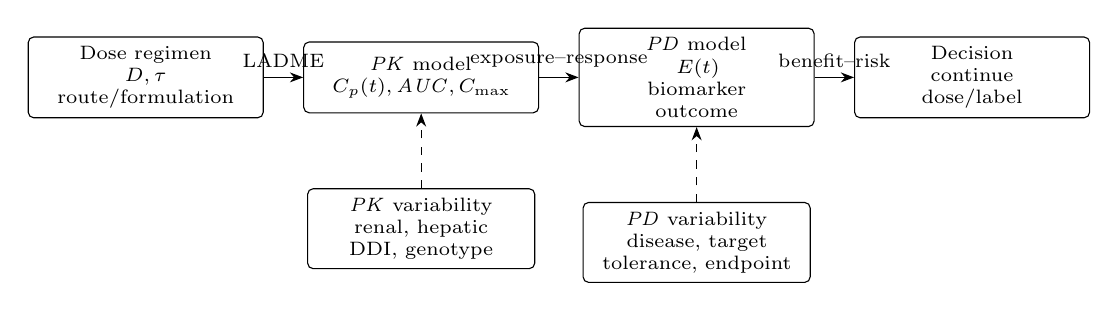
\begin{tikzpicture}[
  node distance=0.5cm,
  box/.style={draw, rounded corners=2pt, align=center, text width=2.75cm, minimum height=0.9cm, font=\scriptsize},
  smallbox/.style={draw, rounded corners=2pt, align=center, text width=2.65cm, minimum height=0.78cm, font=\scriptsize},
  >=Stealth
]
  \node[box] (dose) {Dose regimen\\ \(D,\tau\)\\ route/formulation};
  \node[box, right=of dose] (pk) {\PK{} model\\ \(C_p(t), \AUC, \Cmax\)};
  \node[box, right=of pk] (pd) {\PD{} model\\ \(E(t)\)\\ biomarker\\ outcome};
  \node[box, right=of pd] (decision) {Decision\\ continue\\ dose/label};

  \draw[->] (dose) -- node[above,font=\scriptsize]{LADME} (pk);
  \draw[->] (pk) -- node[above,font=\scriptsize]{exposure--response} (pd);
  \draw[->] (pd) -- node[above,font=\scriptsize]{benefit--risk} (decision);

  \node[smallbox, below=0.95cm of pk] (varpk) {\PK{} variability\\ renal, hepatic\\ DDI, genotype};
  \node[smallbox, below=0.95cm of pd] (varpd) {\PD{} variability\\ disease, target\\ tolerance, endpoint};
  \draw[->, dashed] (varpk) -- (pk);
  \draw[->, dashed] (varpd) -- (pd);
\end{tikzpicture}
}
\captionof{figure}{Lesson 1 的最小工作图。A dose becomes defensible only after exposure, response, uncertainty, and benefit--risk have been connected.}
\end{center}

This is also an inference problem. Before a trial, exposure and response are random quantities:
\[
  \rv{Y}\sim p(y\mid a,\theta),
\]
where \(a\) is the action or design: dose level, sampling scheme, endpoint, inclusion criteria. After observing data \(y\), we update what we believe about \(\theta\), then choose a new action. A 6.437-style decision statement would be
\[
  a^\star
  =
  \argmin_a
  \Ex\!\left[L(a,\Theta,\rv{Y}_{\pklab{future}})\mid \data\right].
\]
In ordinary clinical pharmacology language: use all accumulated data to choose the next dose, next trial, next model, or next label statement.

\begin{remark}
  I visually checked the two original slide decks before redrawing the diagrams in this note.  The figures below are intentionally not raw slide screenshots; they are simplified reconstructions of the teaching visuals in the 1A/1B decks, tuned for LaTeX, PDF, and pdf2htmlEX readability.
\end{remark}

\subsection{Why this belongs at the beginning}

The syllabus objectives for 1A and 1B are not two disconnected lists. The first list says where \PKPD{} is used in clinical drug development; the second list gives the symbols and models that make \PKPD{} usable. The conceptual order is:
\begin{enumerate}[label=\arabic*., leftmargin=2.4em]
  \item development decision;
  \item exposure--response question;
  \item \PK{} and \PD{} parameters;
  \item trial/label decision.
\end{enumerate}

So this note is organized around questions rather than slide order:
\begin{itemize}[leftmargin=2em]
  \item Why do so many drugs fail, and why is insufficient efficacy so common?
  \item What does it mean to ``learn'' rather than merely ``confirm''?
  \item Why is dose selection a scientific and regulatory problem, not just a dosing table?
  \item How do \CL, \Vd, \(t_{1/2}\), \Fbio, \Emax, \ECfifty, and Hill factor enter the decision chain?
  \item What goes wrong when response lags behind concentration?
\end{itemize}

\section{1A: Drug Development as Sequential Learning}

\subsection{Clinical phases are decision points}

The textbook version says Phase 1 is safety and \PK, Phase 2 is efficacy and dose-ranging in patients, Phase 3 is pivotal confirmation, and Phase 4 is post-approval learning. That is true enough to start, but too rigid if taken literally. Cancer, serious infections, and rare diseases often modify the sequence; Phase 1 may occur in patients; Phase 2 and Phase 3 may be combined; adaptive designs may move information across boundaries. The lecture correctly warns that the type and sequence of studies vary by program \cite{ufPha6125Lesson1A2020}.

\begin{center}
\footnotesize
\begin{tabularx}{\textwidth}{p{0.16\textwidth}X X}
\toprule
Stage & Usual development question & How \PKPD{} contributes \\
\midrule
Preclinical &
Is the mechanism plausible enough and safe enough to enter humans? &
In vitro metabolism, transporter work, animal \PKPD, toxicokinetics, first-in-human dose rationale. \\
Phase 1 &
Can humans tolerate the drug, and what exposure results from dose? &
Single/multiple ascending dose, food effect, absorption, \CL, \Vd, \(t_{1/2}\), early biomarkers, PK-guided escalation. \\
Phase 2a &
Is there proof of mechanism and proof of concept in the target biology or disease? &
Target engagement, biomarker response, early exposure--response, whether failure means target failure or inadequate exposure. \\
Phase 2b &
Which dose range should enter pivotal trials? &
Dose-ranging, dose--response models, efficacy/safety tradeoff, simulation of Phase 3 operating characteristics. \\
Phase 3 &
Is there substantial evidence of benefit--risk in the intended population? &
Sparse-sampling \PopPK, exposure--response for clinical outcomes, covariate effects, dose adjustment in subgroups, label support. \\
Phase 4 &
How should use evolve after approval? &
New indications, real-world safety, special populations, formulation changes, postmarketing dose refinement. \\
\bottomrule
\end{tabularx}
\captionof{table}{The phase names are less important than the decisions they support.}
\end{center}

\subsection{Learning versus confirming}

Sheiner's learn/confirm distinction is the intellectual center of 1A \cite{sheiner1997learning}. A confirming trial asks a yes/no question:
\[
  H_0:\Delta \le 0
  \quad\text{versus}\quad
  H_1:\Delta>0.
\]
Does the drug beat placebo or active control on a primary endpoint, at a pre-specified significance level? This is necessary for approval, but it is a poor way to learn the shape of a dose--response curve.

A learning trial asks quantitative questions:
\[
  \begin{gathered}
    \text{How much exposure is needed?}
    \quad
    \text{How steep is the response?}\\
    \text{Where does toxicity begin?}
    \quad
    \text{Which patients need dose adjustment?}
  \end{gathered}
\]
Learning is about estimating a function; confirming is about testing a claim.

\begin{center}
\resizebox{0.92\textwidth}{!}{%
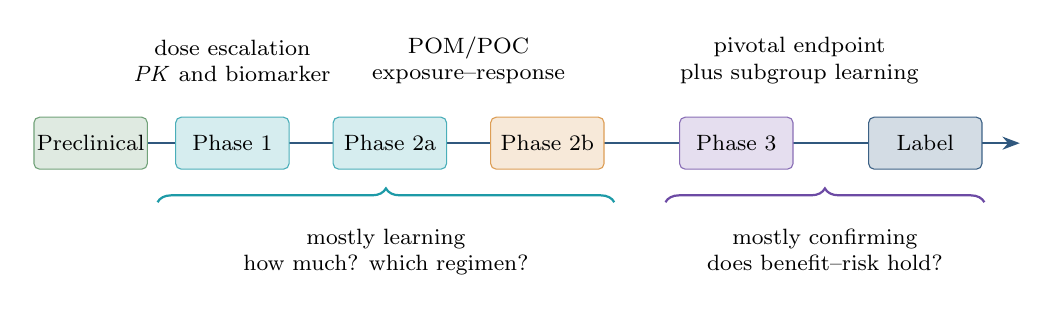
\begin{tikzpicture}[x=1cm,y=1cm]
  \draw[noteArrow] (0,0) -- (12.2,0);
  \foreach \x/\lab/\col in {0.4/{Preclinical}/pkgreen,2.2/{Phase 1}/pkcyan,4.2/{Phase 2a}/pkcyan,6.2/{Phase 2b}/pkorange,8.6/{Phase 3}/pkpurple,11.0/{Label}/pkblue} {
    \draw[fill=\col!18, draw=\col!80, rounded corners=2pt] (\x-0.72,-0.33) rectangle (\x+0.72,0.33);
    \node[font=\footnotesize] at (\x,0) {\lab};
  }
  \draw[decorate, decoration={brace, amplitude=5pt}, thick, draw=pkcyan] (1.25,-0.75) -- (7.05,-0.75)
    node[midway, below=6pt, noteLabel] {mostly learning\\ how much? which regimen?};
  \draw[decorate, decoration={brace, amplitude=5pt}, thick, draw=pkpurple] (7.7,-0.75) -- (11.75,-0.75)
    node[midway, below=6pt, noteLabel] {mostly confirming\\ does benefit--risk hold?};
  \node[noteLabel, text width=3.2cm] at (2.2,1.05) {dose escalation\\ \PK{} and biomarker};
  \node[noteLabel, text width=3.4cm] at (5.2,1.05) {POM/POC\\ exposure--response};
  \node[noteLabel, text width=3.7cm] at (9.4,1.05) {pivotal endpoint\\ plus subgroup learning};
\end{tikzpicture}
}
\captionof{figure}{A redrawn learn/confirm map based on the Lesson 1A slides. Phase 3 confirms the primary claim, but still learns dose adjustment and variability.}
\end{center}

\begin{remark}
  The practical mistake is to design a Phase 2b dose-ranging study as if it were a mini-Phase 3 trial. If each dose arm is powered for pairwise comparison against placebo, the trial may prove that several high doses all work, yet still fail to locate the lowest useful dose or the benefit--risk optimum.
\end{remark}

\subsection{Model-based drug development}

Lalonde et al. describe model-based drug development as a continuum of learn, confirm, and predict, where modeling and simulation are used at each decision point \cite{lalonde2007model}. In 2026 regulatory language, this is now usually called model-informed drug development (\MIDD). FDA's MIDD paired meeting program is built around the use of exposure-based, biological, and statistical models from preclinical and clinical data to support development and regulatory review \cite{fdaMiddProgram2026}. ICH M15 now gives a harmonized framework for MIDD planning, model evaluation, evidence documentation, and the ``question of interest'' \cite{ichM15Midd2026}.

The important update is not just terminology. The modern standard asks:
\[
  \begin{gathered}
    \text{What decision will the model inform,}\\
    \text{and what is the consequence of being wrong?}
  \end{gathered}
\]
If the model only summarizes observed \PK, credibility requirements are modest. If the model replaces a dedicated trial or supports a label dosing recommendation in an unstudied population, model evaluation and documentation must be much stronger.

\section{Attrition, POM/POC, and the Dose-Selection Problem}

\subsection{Clinical attrition is still the background pressure}

The lecture uses the classic ``more than 90\% attrition'' framing. The exact number depends on dataset, time period, modality, and indication, but the qualitative statement remains right: most compounds entering clinical development do not become approved medicines.

Older analyses showed that poor \PK{} and bioavailability were major attrition causes in the early 1990s, then became less dominant as in vitro ADME, formulation, and human \PK{} prediction improved \cite{kola2004attrition}. Later analyses shifted attention toward insufficient efficacy in Phase 2 and Phase 3 \cite{arrowsmith2011phase2,harrison2016phase}. The BIO/Informa/QLS 2011--2020 report estimates overall Phase 1-to-approval likelihoods in the single digits for many categories, with Phase 2 remaining the lowest transition point across most disease areas \cite{bio2021success}.

\begin{center}
\resizebox{0.9\textwidth}{!}{%
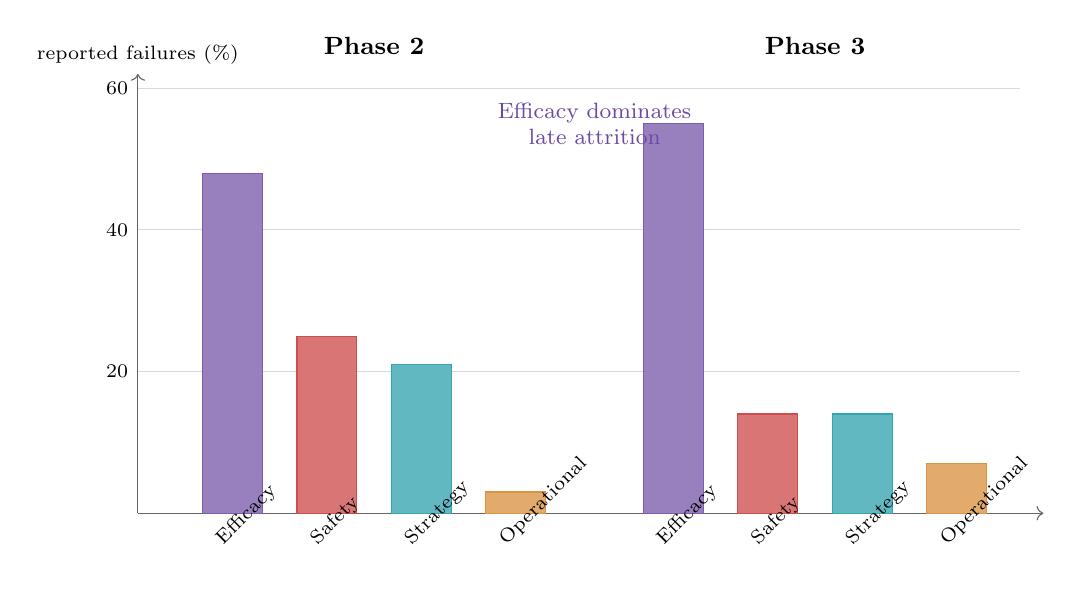
\begin{tikzpicture}[x=1cm,y=0.09cm]
  \draw[->, draw=black!60] (0,0) -- (0,62) node[above,font=\scriptsize]{reported failures (\%)};
  \draw[->, draw=black!60] (0,0) -- (11.5,0);
  \foreach \y in {20,40,60} {
    \draw[draw=black!15] (0,\y) -- (11.2,\y);
    \node[left,font=\scriptsize] at (0,\y) {\y};
  }
  \foreach \x/\h/\col/\lab in {1.2/48/pkpurple/Efficacy,2.4/25/pkred/Safety,3.6/21/pkcyan/Strategy,4.8/3/pkorange/Operational,6.8/55/pkpurple/Efficacy,8.0/14/pkred/Safety,9.2/14/pkcyan/Strategy,10.4/7/pkorange/Operational}{
    \draw[fill=\col!70, draw=\col!90] (\x-0.38,0) rectangle (\x+0.38,\h);
    \node[rotate=45, anchor=west, font=\scriptsize] at (\x-0.25,-5) {\lab};
  }
  \node[font=\small\bfseries] at (3.0,66) {Phase 2};
  \node[font=\small\bfseries] at (8.6,66) {Phase 3};
  \node[align=center, font=\footnotesize, text=pkpurple] at (5.8,55) {Efficacy dominates\\ late attrition};
\end{tikzpicture}
}
\captionof{figure}{Redrawn from the 1A attrition slides: insufficient efficacy remains a central late-development failure mode.}
\end{center}

\begin{warning}
  Attrition statistics should be used as calibration, not fatalism. A drug fails for a reason: wrong target, wrong exposure, wrong endpoint, wrong population, wrong dose, unacceptable safety, commercial redundancy, or simply an insufficiently differentiated benefit. \PKPD{} helps separate these possibilities.
\end{warning}

\subsection{Cost estimates should be handled carefully}

The slide cites a Tufts estimate of about \$2.6B per approved drug. This number is often quoted, but drug development cost is method-sensitive: whether failures are included, how opportunity cost is capitalized, whether the sample is large pharma or smaller firms, and which years are studied all matter. Wouters et al. estimated, using publicly available data for drugs approved from 2009 to 2018, a median capitalized investment of about \$1.14B and a mean of about \$1.56B in 2018 dollars after accounting for failed trials \cite{wouters2020investment}. The honest update is:
\[
  \text{the cost is huge, but no single dollar figure is universal.}
\]

For a pharmacometrician, the point is not the exact dollar amount. It is that wrong learning creates expensive late failure. A weak Phase 2 dose-ranging program can cost years; an incorrect Phase 3 dose can delay approval, force extra trials, or lead to postmarketing dose changes.

\subsection{Proof of mechanism and proof of concept}

Morgan et al. sharpen the early-development problem with the ``three pillars'' of Phase 2 survival: exposure at the site of action, target binding or modulation, and expression of functional pharmacological activity \cite{morgan2012threepillars}. These correspond almost exactly to Lalonde's POM/POC discussion.

\begin{center}
\resizebox{0.86\textwidth}{!}{%
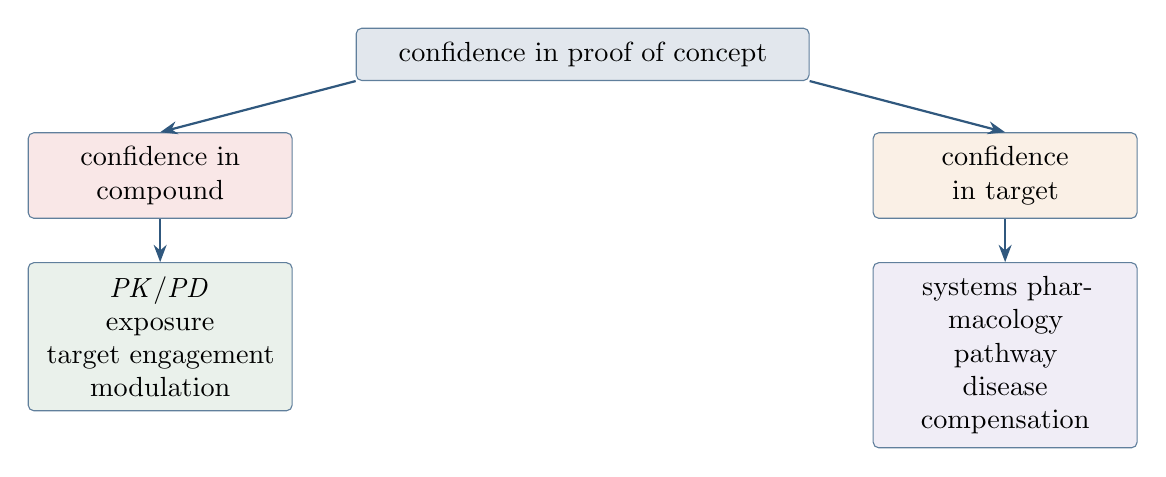
\begin{tikzpicture}[node distance=0.55cm and 0.9cm, >=Stealth]
  \node[noteBox, fill=pkblue!12, text width=5.4cm] (poc) {confidence in proof of concept};
  \node[noteBox, fill=pkred!12, text width=3.0cm, below left=0.65cm and 0.8cm of poc] (compound) {confidence in compound};
  \node[noteBox, fill=pkorange!12, text width=3.0cm, below right=0.65cm and 0.8cm of poc] (target) {confidence in target};
  \node[noteBox, fill=pkgreen!12, text width=3.0cm, below=of compound] (pkpd) {\PKPD\\ exposure\\ target engagement\\ modulation};
  \node[noteBox, fill=pkpurple!10, text width=3.0cm, below=of target] (sys) {systems pharmacology\\ pathway\\ disease\\ compensation};
  \draw[noteArrow] (poc.south west) -- (compound.north);
  \draw[noteArrow] (poc.south east) -- (target.north);
  \draw[noteArrow] (compound) -- (pkpd);
  \draw[noteArrow] (target) -- (sys);
\end{tikzpicture}
}
\captionof{figure}{Redrawn from the POM/POC visual in 1A. \PKPD{} strengthens confidence in the compound; biology determines confidence in the target.}
\end{center}

\begin{center}
\footnotesize
\begin{tabularx}{\textwidth}{p{0.22\textwidth}X X}
\toprule
Question & Evidence & Bad interpretation if missing \\
\midrule
Did the drug reach the site of action? &
Plasma \PK, tissue \PK{} where possible, \PBPK, imaging, CSF or target-site sampling. &
Calling a target ineffective when the drug never reached adequate exposure. \\
Did it engage the target? &
Receptor occupancy, enzyme inhibition, pathway biomarker, target modulation. &
Calling a compound inactive when dose or formulation never tested the mechanism. \\
Did target engagement move biology? &
Functional biomarker, proximal \PD, disease-relevant pathway readout. &
Repeating chemistry around a target whose human biology may not produce therapeutic benefit. \\
\bottomrule
\end{tabularx}
\captionof{table}{POM/POC as a de-risking logic.}
\end{center}

The phrase ``fail with confidence'' is important. A negative POC study is informative only if adequate exposure and mechanism engagement were demonstrated. Otherwise the result is ambiguous:
\[
  \begin{gathered}
    \text{negative clinical response}
    =
    \text{target failed}\\
    \text{or}\\
    \text{compound/dose/formulation failed}.
  \end{gathered}
\]
The purpose of early \PKPD{} is to remove the second explanation as much as possible.

\subsection{The dose is a strategic position on two curves}

The lecture's idealized dose--response figure has an efficacy curve and a safety curve. That picture is deceptively simple. Selecting a dose means selecting a point on a benefit--risk surface:
\[
  U(d)
  =
  \text{benefit}(d)
  -
  \lambda\,\text{harm}(d),
\]
where \(\lambda\) encodes disease severity, available alternatives, patient tolerance, and regulatory judgment. The ``right'' dose for allergic rhinitis may be a safety-differentiated dose; the ``right'' dose for a rapidly fatal disease may sit much closer to the efficacy plateau if toxicity is acceptable.

\begin{center}
\resizebox{0.88\textwidth}{!}{%
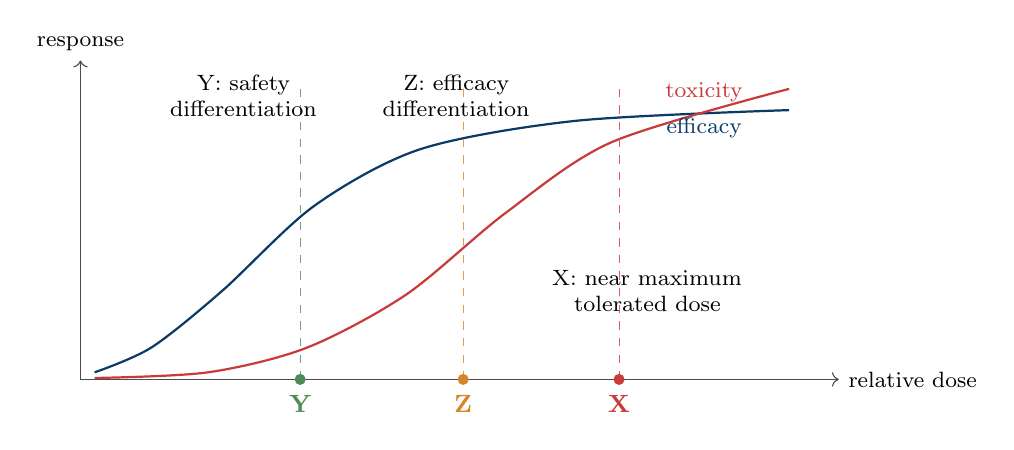
\begin{tikzpicture}[x=0.9cm,y=0.9cm]
  \draw[->, draw=black!70] (0,0) -- (10.7,0) node[right,font=\footnotesize]{relative dose};
  \draw[->, draw=black!70] (0,0) -- (0,4.5) node[above,font=\footnotesize]{response};
  \draw[thick, draw=pkblue] plot[smooth] coordinates {(0.2,0.1) (1,0.45) (2,1.25) (3.3,2.45) (4.8,3.25) (7,3.65) (10,3.8)};
  \draw[thick, draw=pkred] plot[smooth] coordinates {(0.2,0.02) (1.8,0.1) (3.2,0.45) (4.6,1.2) (6,2.35) (7.5,3.35) (10,4.1)};
  \node[text=pkblue,font=\footnotesize] at (8.8,3.55) {efficacy};
  \node[text=pkred,font=\footnotesize] at (8.8,4.05) {toxicity};
  \foreach \x/\lab/\col in {3.1/Y/pkgreen,5.4/Z/pkorange,7.6/X/pkred} {
    \draw[dashed, draw=\col!80] (\x,0) -- (\x,4.15);
    \fill[\col] (\x,0) circle (2pt);
    \node[font=\small\bfseries, text=\col] at (\x,-0.35) {\lab};
  }
  \node[noteLabel, text width=2.4cm] at (2.3,4.0) {Y: safety\\ differentiation};
  \node[noteLabel, text width=2.6cm] at (5.3,4.0) {Z: efficacy\\ differentiation};
  \node[noteLabel, text width=2.6cm] at (8.0,1.25) {X: near maximum\\ tolerated dose};
\end{tikzpicture}
}
\captionof{figure}{Redrawn from the 1A dose-selection slide.  Dose choice is not ``largest tolerated dose'' by default; it is a position on efficacy and safety curves.}
\end{center}

ICH E4 already made this point in 1994: dose--response information helps choose starting dose, titration, maximum useful dose, and labeling instructions; historically, some drugs were marketed at excessive plateau doses \cite{ichE4DoseResponse}. The 2024 FDA Project Optimus guidance in oncology pushes the same principle into a field that traditionally used maximum tolerated dose logic: for molecularly targeted and immune therapies, dose selection should optimize efficacy, safety, and tolerability rather than automatically chase the highest tolerated dose \cite{fda2024projectOptimus}.

\subsection{Dose selection can delay approval}

Sacks et al. reviewed first-cycle failures of new drug applications submitted to FDA from 2000 to 2012 and found dose-selection uncertainty among preventable deficiencies \cite{sacks2014delay}. This is the regulatory mirror of the scientific problem. If Phase 2 does not learn the dose--response relationship, Phase 3 may confirm the wrong thing, or confirm nothing.

The practical rule from the lecture is worth preserving:
\begin{itemize}[leftmargin=2em]
  \item Use a wide enough dose range, often at least 10-fold when feasible.
  \item Prefer more dose levels with fewer subjects per dose when the goal is learning curve shape.
  \item Analyze dose response with regression/modeling, not only pairwise tests.
  \item Separate ``the drug has some activity'' from ``we know the dose for Phase 3.''
\end{itemize}

\section{The Label Is the Final Knowledge Product}

\subsection{Why labeling appears in Lesson 1}

The first slide example of prescribing information is not decorative. It tells us where clinical pharmacology knowledge ends up. FDA's clinical pharmacology labeling guidance states that section 12 contains Mechanism of Action, Pharmacodynamics, and Pharmacokinetics, with Microbiology and Pharmacogenomics subsections when appropriate \cite{fda2016clinicalPharmLabel}. But \PKPD{} also informs other label sections:
\begin{itemize}[leftmargin=2em]
  \item Dosage and Administration: dose, interval, titration, maximum dose, missed dose, formulation.
  \item Drug Interactions: CYPs, transporters, protein binding, additive \PD{} toxicity, antagonism.
  \item Use in Specific Populations: renal impairment, hepatic impairment, pregnancy, lactation, pediatrics, geriatrics.
  \item Warnings and Precautions: exposure-related toxicity, QT prolongation, bleeding risk, immune toxicity.
  \item Clinical Studies: dose arms, endpoint interpretation, subgroup evidence.
\end{itemize}

\subsection{A label statement is a compressed model}

When a label says ``reduce the dose in severe renal impairment,'' it is hiding a chain of reasoning:
\[
  \text{renal function}
  \rightarrow
  \CL{}
  \rightarrow
  \AUC{}
  \rightarrow
  \text{safety/efficacy}
  \rightarrow
  \text{dose adjustment}.
\]
When a label says ``no dose adjustment is required,'' it hides the same chain but reaches the opposite decision. This is why Phase 3 learning analyses matter: they support not only when adjustment is needed, but also when it is not needed.

\section{1B: PK Begins with LADME}

\subsection{LADME as a causal sequence}

Cristofoletti's 1B lecture begins with LADME: liberation, absorption, distribution, metabolism, excretion \cite{ufPha6125Lesson1B2020}. These are not five vocabulary words; they are five possible rate-limiting steps.

\begin{center}
\footnotesize
\begin{tabularx}{\textwidth}{p{0.18\textwidth}X X}
\toprule
Process & What it means & Common parameter or model role \\
\midrule
Liberation & Drug is released from dosage form. & Dissolution rate, formulation lag, modified release. \\
Absorption & Drug crosses membranes into systemic circulation. & \(\ka\), \Fbio, first-pass extraction, transporters. \\
Distribution & Drug moves between blood and tissues. & \Vd, compartments, tissue partition, protein binding. \\
Metabolism & Drug is enzymatically transformed. & Hepatic \CL, \(\CL_{\pklab{int}}\), CYP effects, nonlinear saturation. \\
Excretion & Drug/metabolites leave the body. & Renal \CL, biliary excretion, transporter-mediated secretion. \\
\bottomrule
\end{tabularx}
\captionof{table}{LADME as a map of where the concentration--time profile can be shaped.}
\end{center}

\begin{center}
\resizebox{0.78\textwidth}{!}{%
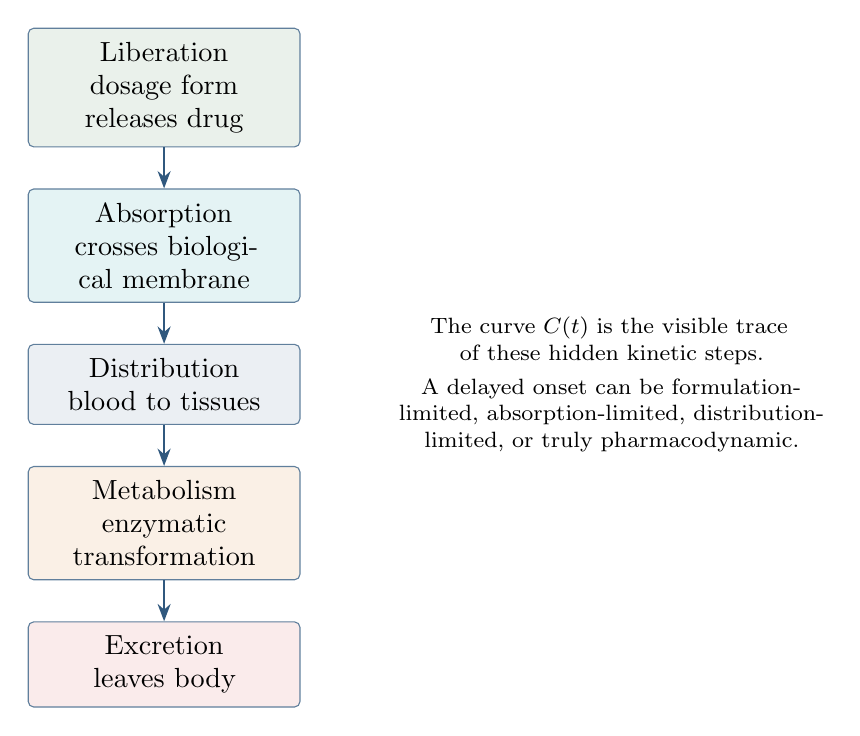
\begin{tikzpicture}[node distance=0.52cm, >=Stealth]
  \node[noteBox, fill=pkgreen!12, text width=3.1cm] (lib) {Liberation\\ dosage form releases drug};
  \node[noteBox, fill=pkcyan!12, text width=3.1cm, below=of lib] (abs) {Absorption\\ crosses biological membrane};
  \node[noteBox, fill=pkblue!8, text width=3.1cm, below=of abs] (dist) {Distribution\\ blood to tissues};
  \node[noteBox, fill=pkorange!12, text width=3.1cm, below=of dist] (met) {Metabolism\\ enzymatic transformation};
  \node[noteBox, fill=pkred!10, text width=3.1cm, below=of met] (exc) {Excretion\\ leaves body};
  \foreach \a/\b in {lib/abs,abs/dist,dist/met,met/exc} \draw[noteArrow] (\a) -- (\b);
  \node[noteLabel, text width=5.4cm, right=1.1cm of dist] {
    The curve \(C(t)\) is the visible trace of these hidden kinetic steps.\\[3pt]
    A delayed onset can be formulation-limited, absorption-limited, distribution-limited, or truly pharmacodynamic.
  };
\end{tikzpicture}
}
\captionof{figure}{Redrawn from the 1B LADME slide as a causal flow rather than a vocabulary list.}
\end{center}

\subsection{A PK experiment}

A minimal \PK{} study has four steps:
\[
  \begin{gathered}
    \text{administer dose}
    \rightarrow
    \text{sample fluids over time}\\
    \rightarrow
    \text{measure concentration}
    \rightarrow
    \text{estimate parameters}.
  \end{gathered}
\]
The sampled fluid is often plasma or whole blood; sometimes urine, saliva, CSF, or tissue is relevant. The measurement method may be LC--MS/MS for small molecules or immunoassay for biologics. But the conceptual output is always a time series:
\[
  (t_1,C_1),\ldots,(t_n,C_n).
\]

There are two broad analysis styles:
\begin{itemize}[leftmargin=2em]
  \item \NCA: compute summaries such as \(\AUC\), \(\Cmax\), \(\Tmax\), \(t_{1/2}\), \(\CL\), and \(\Vd\) using limited structural assumptions.
  \item Model-based analysis: posit differential equations or statistical models that can simulate unobserved concentrations, covariate effects, and future dosing regimens.
\end{itemize}
``Model independent'' is a convenient phrase, but \NCA{} still assumes enough linearity and accessible elimination for its summaries to be meaningful.

\section{Clearance}

\subsection{Why clearance has units of volume per time}

Clearance quantifies elimination. The first-order elimination idea is:
\[
  \frac{\dd A}{\dd t}=-\ke{} A,
\]
where \(A\) is amount in the body. If \(A=\Vd{} C\), then
\[
  -\frac{\dd A}{\dd t}=\ke{} \Vd{} C.
\]
Define clearance as the proportionality between rate of elimination and concentration:
\[
  \text{rate}_{\pklab{elim}} = \CL\,C,
  \qquad
  \CL=\ke{} \Vd.
\]
This is why \CL{} has units of volume/time. It is not literally a bucket of blood being cleaned; it is a proportionality constant that converts concentration into elimination rate.

\begin{remark}
  The lecture asks why we do not use mg/h as the elimination parameter. Because for first-order elimination, mg/h changes with concentration. \CL{} is useful because it is often approximately constant over the therapeutic range.
\end{remark}

\subsection{Clearance is usually additive}

Total clearance can be decomposed:
\[
  \CL_{\pklab{T}}
  =
  \CL_{\pklab{renal}}
  +
  \CL_{\pklab{hepatic}}
  +
  \CL_{\pklab{other}}.
\]
This is bookkeeping with physiological meaning. If renal clearance falls because kidney function declines, total clearance falls unless another pathway compensates. If metabolism is saturated, \CL{} may no longer be constant. Phenytoin is the standard classroom example: therapeutic concentrations can approach the nonlinear Michaelis--Menten region.

\subsection{Organ clearance and extraction}

For an eliminating organ with blood flow \(Q\), incoming concentration \(C_A\), and outgoing concentration \(C_V\), mass balance gives
\[
  \text{rate}_{\pklab{extracted}} = Q(C_A-C_V).
\]
The extraction ratio is
\[
  E=\frac{C_A-C_V}{C_A}.
\]
Organ clearance is then
\[
  \CL_{\pklab{organ}}=Q E.
\]

\begin{center}
\resizebox{0.74\textwidth}{!}{%
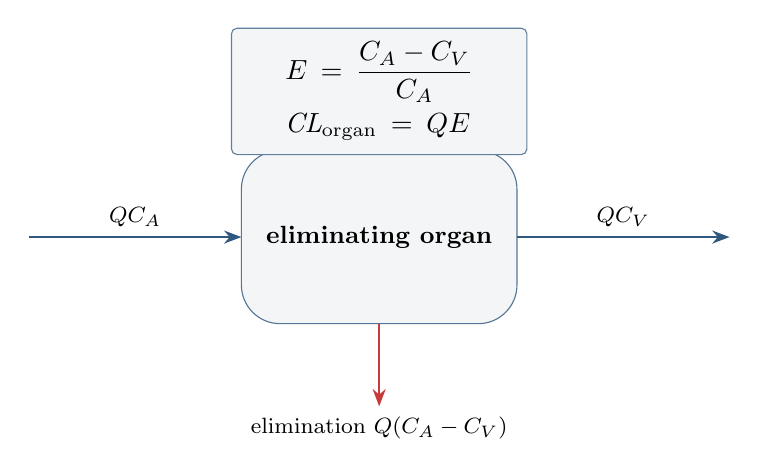
\begin{tikzpicture}[x=1cm,y=1cm]
  \draw[fill=pkgray, draw=pkblue!70, rounded corners=14pt] (3,0.5) rectangle (6.5,2.7);
  \node[font=\small\bfseries] at (4.75,1.6) {eliminating organ};
  \draw[noteArrow] (0.3,1.6) -- (3,1.6) node[midway, above, font=\footnotesize] {\(Q C_A\)};
  \draw[noteArrow] (6.5,1.6) -- (9.2,1.6) node[midway, above, font=\footnotesize] {\(Q C_V\)};
  \draw[noteArrow, draw=pkred] (4.75,0.5) -- (4.75,-0.55) node[below, font=\footnotesize] {elimination \(Q(C_A-C_V)\)};
  \node[noteBox, text width=3.4cm] at (4.75,3.45) {\(\displaystyle E=\frac{C_A-C_V}{C_A}\)\\[3pt]\(\displaystyle \CL_{\pklab{organ}}=QE\)};
\end{tikzpicture}
}
\captionof{figure}{Redrawn from the organ-clearance slides: clearance can be seen as blood flow times extraction efficiency.}
\end{center}

For the well-stirred liver model,
\[
  \CL_{\pklab{H,B}}
  =
  Q_H
  \frac{f_{u,B}\CL_{\pklab{int}}}
       {Q_H+f_{u,B}\CL_{\pklab{int}}}.
\]
Two limiting cases are the whole intuition:
\[
  \begin{aligned}
    \text{high extraction:}\quad
    f_{u,B}\CL_{\pklab{int}}\gg Q_H
    &\Rightarrow
    \CL_{\pklab{H,B}}\approx Q_H,\\
    \text{low extraction:}\quad
    f_{u,B}\CL_{\pklab{int}}\ll Q_H
    &\Rightarrow
    \CL_{\pklab{H,B}}\approx f_{u,B}\CL_{\pklab{int}}.
  \end{aligned}
\]
High-extraction drugs are flow-limited; low-extraction drugs are limited by intrinsic capacity and protein binding. This distinction predicts how hepatic blood flow, enzyme inhibition, induction, and binding changes affect exposure.

\subsection{Blood, plasma, and unbound clearance}

The fluid matters. If concentrations are measured in plasma but the organ sees whole blood, one must convert:
\[
  \CL_B C_B=\CL_P C_P.
\]
Similarly, if only unbound drug is pharmacologically and metabolically available, then unbound clearance is a different descriptor:
\[
  \CL_u C_u=\CL{} C.
\]
This is not cosmetic. A high plasma-protein-binding drug can have small total unbound fraction but still high intrinsic clearance of unbound drug. Always ask: clearance with respect to what concentration?

\section{Volume, Half-Life, Bioavailability, and Absorption}

\subsection{Apparent volume of distribution}

The apparent volume of distribution relates amount in the body to measured concentration:
\[
  \Vd=\frac{A_{\pklab{body}}}{C}.
\]
The word ``apparent'' does a lot of work. \Vd{} is not necessarily an anatomical space. If concentration in plasma is low because drug partitions into tissue, \Vd{} can be far larger than body water. That is why azithromycin can have an enormous apparent \Vd, while gentamicin approximates extracellular fluid.

\begin{center}
\resizebox{0.82\textwidth}{!}{%
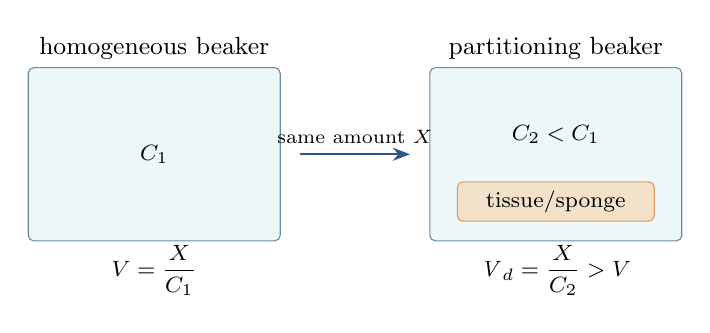
\begin{tikzpicture}[x=1cm,y=1cm]
  \draw[fill=pkcyan!8, draw=pkblue!60, rounded corners=2pt] (0,0) rectangle (3.2,2.2);
  \node[font=\small] at (1.6,2.45) {homogeneous beaker};
  \node[font=\footnotesize] at (1.6,1.1) {\(C_1\)};
  \node[font=\footnotesize] at (1.6,-0.38) {\(\displaystyle V=\frac{X}{C_1}\)};
  \draw[fill=pkcyan!8, draw=pkblue!60, rounded corners=2pt] (5.1,0) rectangle (8.3,2.2);
  \draw[fill=pkorange!25, draw=pkorange!80, rounded corners=2pt] (5.45,0.25) rectangle (7.95,0.75);
  \node[font=\small] at (6.7,2.45) {partitioning beaker};
  \node[font=\footnotesize] at (6.7,1.35) {\(C_2<C_1\)};
  \node[font=\footnotesize] at (6.7,0.5) {tissue/sponge};
  \node[font=\footnotesize] at (6.7,-0.38) {\(\displaystyle \Vd=\frac{X}{C_2}>V\)};
  \draw[noteArrow] (3.45,1.1) -- (4.85,1.1) node[midway, above, font=\scriptsize]{same amount \(X\)};
\end{tikzpicture}
}
\captionof{figure}{Redrawn from the 1B sponge/beaker slide.  Apparent volume grows when measured concentration is low because drug has partitioned outside the sampled fluid.}
\end{center}

\begin{remark}
  A high \Vd{} often says: the drug is somewhere else, not mainly in plasma. It does not say the body has that many liters of fluid.
\end{remark}

\subsection{Half-life is secondary}

For first-order elimination,
\[
  t_{1/2}=\frac{\log 2}{\ke}
  =
  \frac{\log 2\,\Vd}{\CL}.
\]
This is why half-life is a hybrid parameter. It changes if \Vd{} changes, if \CL{} changes, or both. Obesity may increase \Vd{} for lipophilic drugs; renal or hepatic impairment may decrease \CL; either can lengthen \(t_{1/2}\).

The common beginner error is to treat half-life as if it alone determines dosing. It does not. Dosing depends on target exposure, therapeutic window, fluctuation tolerance, onset, adherence, formulation, and response delay. Half-life tells us about decline; it does not by itself define the right regimen.

\subsection{Bioavailability}

Absolute bioavailability is the fraction of an extravascular dose reaching systemic circulation:
\[
  \Fbio{}
  =
  \frac{\AUC_{\pklab{EV}}/D_{\pklab{EV}}}
       {\AUC_{\pklab{IV}}/D_{\pklab{IV}}}.
\]
For oral dosing, low \Fbio{} may reflect incomplete dissolution, poor permeability, gut metabolism, efflux transport, or hepatic first-pass metabolism. The daclatasvir stable-isotope microdose example in the lecture is a beautiful design idea: give oral unlabeled drug and IV isotopically labeled microdose together, then use mass spectrometry to distinguish them, reducing intersubject and interoccasion variability.

\subsection{AUC and the trapezoidal rule}

\(\AUC\) is exposure:
\[
  \AUC_{0-t_{\pklab{last}}}
  \approx
  \sum_{i=1}^{n-1}
  \frac{C_i+C_{i+1}}{2}(t_{i+1}-t_i).
\]
The tail is often approximated by
\[
  \AUC_{t_{\pklab{last}}-\infty}
  =
  \frac{C_{\pklab{last}}}{\kel}.
\]
If too much of total \(\AUC\) comes from extrapolation, the profile was not sampled long enough. Cristofoletti gives the practical criterion that \(\AUC_{0-t}/\AUC_{0-\infty}\) should ideally exceed about 80\%.

\subsection{Absorption rate}

The syllabus explicitly asks for absorption rate. In the simplest first-order oral absorption model:
\[
  \frac{\dd A_g}{\dd t}=-\ka{} A_g,
  \qquad
  \frac{\dd A_c}{\dd t}=\Fbio\ka{} A_g-\frac{\CL}{\Vd}A_c.
\]
For a single extravascular dose with one-compartment disposition and \(\ka\ne \ke\),
\[
  C(t)
  =
  \frac{\Fbio{} D\ka}{\Vd(\ka-\ke)}
  \left(e^{-\ke{} t}-e^{-\ka{} t}\right).
\]
\(\ka\) controls how fast drug enters systemic circulation. It affects \(\Tmax\), \(\Cmax\), early exposure, and therefore onset. For acute pain, a slow or erratic absorption phase can make a good molecule look weak because the response window is early.

\section{PD Parameters and Empirical Models}

\subsection{Effect, efficacy, and baseline}

Cristofoletti separates three words:
\begin{itemize}[leftmargin=2em]
  \item Effect: drug-induced change in a physiological parameter relative to baseline.
  \item Efficacy: therapeutically beneficial effect, often integrating multiple effects.
  \item Baseline: physiological state without drug.
\end{itemize}
This distinction matters because a biomarker effect is not automatically clinical efficacy. A drug may strongly lower a biomarker yet fail to improve outcomes; conversely, a clinical endpoint may respond slowly even if the proximal biomarker moves quickly.

\subsection{The sigmoid Emax model}

The most common empirical concentration--response model is
\[
  E(C)
  =
  E_0
  +
  \frac{\Emax{} C^n}{\ECfifty^n+C^n}.
\]
\(E_0\) is baseline, \(\Emax\) is maximal drug effect above baseline, \(\ECfifty\) is potency in the system, and \(n\) is the Hill factor controlling steepness. When \(n=1\), this becomes the simple \(\Emax\) model:
\[
  E(C)=E_0+\frac{\Emax{} C}{\ECfifty+C}.
\]

\begin{center}
\resizebox{0.82\textwidth}{!}{%
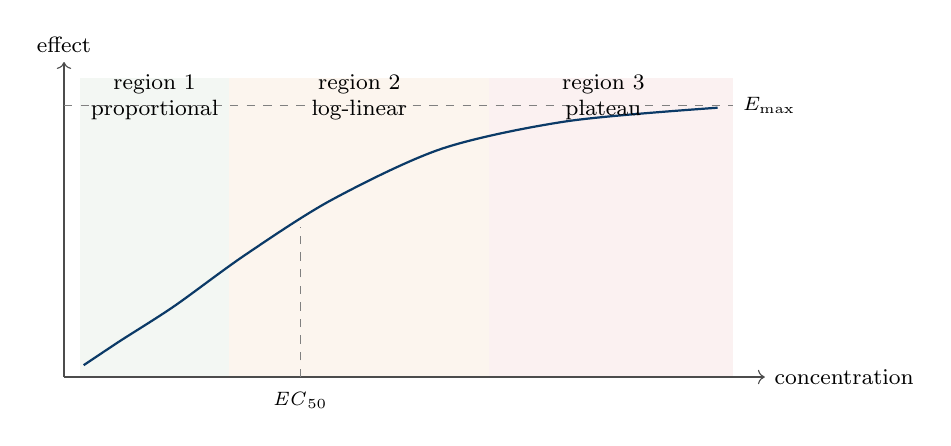
\begin{tikzpicture}[x=1cm,y=1cm]
  \draw[fill=pkgreen!7, draw=none] (0.2,0) rectangle (2.1,3.8);
  \draw[fill=pkorange!8, draw=none] (2.1,0) rectangle (5.4,3.8);
  \draw[fill=pkred!7, draw=none] (5.4,0) rectangle (8.5,3.8);
  \draw[->, draw=black!70] (0,0) -- (8.9,0) node[right,font=\footnotesize]{concentration};
  \draw[->, draw=black!70] (0,0) -- (0,4.0) node[above,font=\footnotesize]{effect};
  \draw[thick, draw=pkblue] plot[smooth] coordinates {(0.25,0.15) (0.7,0.45) (1.4,0.9) (2.3,1.55) (3.4,2.25) (4.8,2.9) (6.4,3.25) (8.3,3.42)};
  \draw[dashed, draw=black!50] (0,3.45) -- (8.5,3.45) node[right,font=\scriptsize]{\(\Emax\)};
  \draw[dashed, draw=black!50] (3.0,0) -- (3.0,1.9);
  \node[font=\scriptsize] at (3.0,-0.3) {\(\ECfifty\)};
  \node[noteLabel] at (1.15,3.55) {region 1\\ proportional};
  \node[noteLabel] at (3.75,3.55) {region 2\\ log-linear};
  \node[noteLabel] at (6.85,3.55) {region 3\\ plateau};
\end{tikzpicture}
}
\captionof{figure}{Redrawn from the 1B \(\Emax\) slides.  The curve is one object, but different approximations are useful in different concentration regions.}
\end{center}

Three regions are worth memorizing:
\begin{itemize}[leftmargin=2em]
  \item Low concentration: response is approximately proportional to \(C\).
  \item Middle region: response is often close to linear in \(\log C\).
  \item High concentration: response approaches a plateau; more exposure gives diminishing returns.
\end{itemize}

\subsection{A small model table}

\begin{center}
\footnotesize
\begin{tabularx}{\textwidth}{p{0.22\textwidth}X X}
\toprule
Model & Formula & Use \\
\midrule
Linear &
\(E=E_0+sC\) &
Low-concentration approximation; no plateau observed. \\
Log-linear &
\(E=a+b\log C\) &
Middle part of an \(\Emax\)-like curve; useful for local thinking. \\
\(\Emax\) &
\(E=E_0+\Emax{} C/(\ECfifty+C)\) &
Saturable response with Hill factor \(n=1\). \\
Sigmoid \(\Emax\) &
\(E=E_0+\Emax{} C^n/(\ECfifty^n+C^n)\) &
Steeper or shallower transition; empirical workhorse. \\
Inhibitory \(\Emax\) &
\(E=E_0-\Imax{} C^n/(\ICfifty^n+C^n)\) &
Drug reduces a baseline quantity, e.g. enzyme activity or viral load. \\
\bottomrule
\end{tabularx}
\captionof{table}{Empirical \PD{} models. \(\Imax\) and \(\ICfifty\) are inhibitory analogues of \(\Emax\) and \(\ECfifty\).}
\end{center}

\subsection{When Emax is not enough}

Derendorf and Meibohm emphasize that \PKPD{} modeling links dose--concentration and concentration--effect relationships to describe and predict the time course of drug effects \cite{derendorf1999modeling}. But a direct \(C(t)\mapsto E(t)\) plug-in only works when the effect site equilibrates quickly and the response mechanism is immediate:
\[
  E(t)=E_0+\frac{\Emax{} C_p(t)^n}{\ECfifty^n+C_p(t)^n}.
\]
When there is temporal dissociation, this direct model becomes wrong in a specific way: the same plasma concentration can correspond to two different effects depending on whether concentration is rising or falling. That loop is hysteresis.

\section{Time Delays and Rate-Limiting Steps}

\subsection{Counter-clockwise hysteresis}

Ibuprofen's antipyretic effect peaks later than plasma concentration. If one plots effect against plasma concentration, the curve loops counter-clockwise: at the same \(C_p\), effect is smaller on the way up and larger later. The interpretation is not mystical; response is downstream of mediator turnover. The drug reduces prostaglandin production, but existing mediators and heat balance take time to change.

\begin{center}
\resizebox{0.82\textwidth}{!}{%
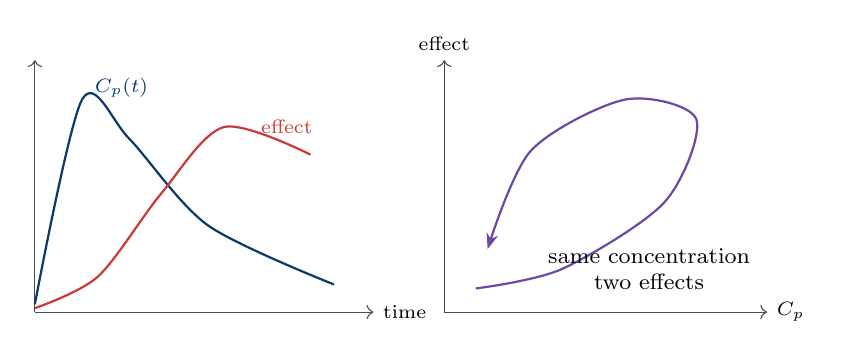
\begin{tikzpicture}[x=1cm,y=1cm]
  \begin{scope}
    \draw[->, draw=black!70] (0,0) -- (4.3,0) node[right,font=\scriptsize]{time};
    \draw[->, draw=black!70] (0,0) -- (0,3.2);
    \draw[thick, draw=pkblue] plot[smooth] coordinates {(0,0.1) (0.6,2.7) (1.2,2.2) (2.2,1.1) (3.8,0.35)};
    \draw[thick, draw=pkred] plot[smooth] coordinates {(0,0.05) (0.8,0.45) (1.6,1.5) (2.4,2.35) (3.5,2.0)};
    \node[text=pkblue,font=\scriptsize] at (1.1,2.85) {\(C_p(t)\)};
    \node[text=pkred,font=\scriptsize] at (3.2,2.35) {effect};
  \end{scope}
  \begin{scope}[shift={(5.2,0)}]
    \draw[->, draw=black!70] (0,0) -- (4.1,0) node[right,font=\scriptsize]{\(C_p\)};
    \draw[->, draw=black!70] (0,0) -- (0,3.2) node[above,font=\scriptsize]{effect};
    \draw[thick, draw=pkpurple, -{Stealth[length=2mm]}] plot[smooth] coordinates {(0.4,0.3) (1.5,0.55) (2.8,1.4) (3.2,2.45) (2.3,2.7) (1.1,2.05) (0.55,0.8)};
    \node[noteLabel, text width=2.6cm] at (2.6,0.55) {same concentration\\ two effects};
  \end{scope}
\end{tikzpicture}
}
\captionof{figure}{Redrawn from the ibuprofen hysteresis slide.  A delayed response produces a loop when effect is plotted against plasma concentration.}
\end{center}

A common fix is an effect compartment:
\[
  \frac{\dd C_e}{\dd t}=k_{e0}(C_p-C_e),
  \qquad
  E(t)=E(C_e(t)).
\]
This says the effect site concentration \(C_e\) lags behind plasma. It is a phenomenological delay model; it may or may not correspond to a literal compartment.

\subsection{Turnover models}

For indirect response, the drug acts on production or loss of an endogenous mediator:
\[
  \frac{\dd R}{\dd t}
  =
  k_{\pklab{in}}\cdot S(C)
  -
  k_{\pklab{out}}\cdot R,
\]
or
\[
  \frac{\dd R}{\dd t}
  =
  k_{\pklab{in}}
  -
  k_{\pklab{out}}\cdot I(C)\,R.
\]
Here \(S(C)\) may stimulate input and \(I(C)\) may inhibit output, depending on mechanism. Aspirin is an extreme teaching example: plasma aspirin disappears quickly, but platelet thromboxane recovery can take days because aspirin irreversibly inhibits platelet cyclooxygenase and platelets cannot synthesize new enzyme. The rate-limiting step is biological replacement, not plasma elimination.

Felmlee, Morris, and Mager organize these mechanism-based \PD{} models into direct effects, biophase distribution, indirect response, signal transduction, and irreversible effects \cite{felmlee2012mechanism}. That taxonomy is a useful preview of later modules.

\subsection{The rate-limiting-step question}

Whenever concentration and response are disconnected, ask:
\[
  \begin{gathered}
    \text{What is the slowest step}\\
    \text{between plasma concentration and observed response?}
  \end{gathered}
\]
Candidate answers include:
\begin{itemize}[leftmargin=2em]
  \item absorption or formulation release,
  \item distribution to the site of action,
  \item receptor binding or target turnover,
  \item endogenous mediator turnover,
  \item signal transduction cascade,
  \item cell turnover or disease progression,
  \item tolerance, adaptation, or feedback.
\end{itemize}
This question determines whether to use direct effect, effect compartment, indirect response, transit compartments, irreversible inhibition, or disease-progression models.

\section{Case Study: SC-75416 and Acute Pain}

\subsection{What the naive read would conclude}

The SC-75416 example is pedagogically important because it shows how \PK{} data can rescue interpretation. In a dental pain Phase 2 POC study, capsule SC-75416 produced less pain relief than expected, while the active control worked. A naive efficacy-only read would say: the drug has insufficient efficacy.

But \PK{} showed lower and erratic early exposure for the capsule. For acute pain, early exposure is the response window. The causal interpretation changes:
\[
  \text{weak observed pain relief}
  \ne
  \text{weak molecule}
\]
if the formulation failed to generate adequate early exposure.

\begin{center}
\resizebox{0.82\textwidth}{!}{%
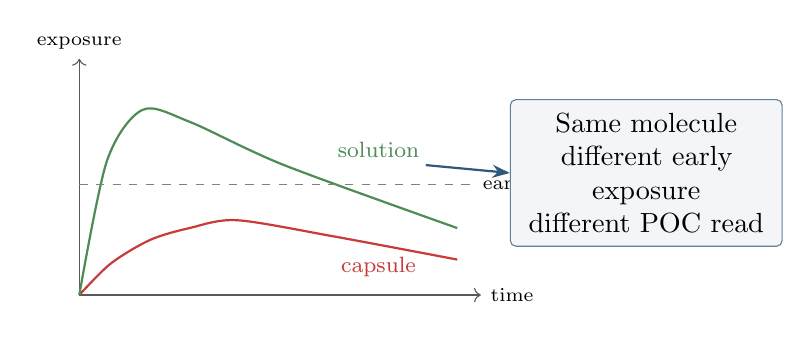
\begin{tikzpicture}[x=1cm,y=1cm]
  \begin{scope}
    \draw[->, draw=black!65] (0,0) -- (5.1,0) node[right,font=\scriptsize]{time};
    \draw[->, draw=black!65] (0,0) -- (0,3.0) node[above,font=\scriptsize]{exposure};
    \draw[thick, draw=pkred] plot[smooth] coordinates {(0,0) (0.4,0.4) (0.9,0.7) (1.4,0.85) (2.0,0.95) (3.2,0.75) (4.8,0.45)};
    \draw[thick, draw=pkgreen] plot[smooth] coordinates {(0,0) (0.35,1.7) (0.8,2.35) (1.4,2.2) (2.6,1.65) (4.8,0.85)};
    \draw[dashed, draw=black!50] (0,1.4) -- (5,1.4) node[right,font=\scriptsize]{early target};
    \node[text=pkred,font=\footnotesize] at (3.8,0.35) {capsule};
    \node[text=pkgreen,font=\footnotesize] at (3.8,1.85) {solution};
  \end{scope}
  \node[noteBox, text width=3.1cm] (box) at (7.2,1.55) {Same molecule\\ different early exposure\\ different POC read};
  \draw[noteArrow] (4.4,1.65) -- (box.west);
\end{tikzpicture}
}
\captionof{figure}{Redrawn from the SC-75416 slides: a formulation problem can masquerade as insufficient efficacy when the clinical response window is early.}
\end{center}

\subsection{What the model did}

The \PKPD{} model related dose, concentration, pain relief score, placebo/time effects, and dropout/remedication time. Clinical trial simulations explored what would happen with a faster, more bioavailable oral solution and different dose arms. The model predicted that a 360 mg oral solution dose could be superior to ibuprofen; the subsequent trial supported the prediction \cite{kowalski2008sc75416}.

The lesson is not that models are magic. The lesson is that a model made the ambiguity explicit:
\[
  \text{Is the drug ineffective, or was the exposure profile wrong?}
\]
Without \PK, one might kill a viable mechanism. Without \PD{} and trial simulation, one might overreact to a formulation artifact.

\section{Modern Regulatory Frame}

\subsection{Exposure-response guidance}

FDA's exposure--response guidance recommends using exposure--response information in IND, NDA, and BLA development and explicitly links it with ICH E4 dose--response thinking \cite{fda2003exposureResponse}. In practical terms, the guidance family asks sponsors to connect:
\[
  \text{dose}
  \rightarrow
  \text{exposure}
  \rightarrow
  \text{efficacy and safety}
  \rightarrow
  \text{dose recommendation}.
\]
This is precisely the Lesson 1 diagram.

\subsection{Population PK guidance}

FDA's 2022 Population PK guidance states that population \PK{} analysis is frequently used to guide drug development and inform therapeutic individualization, including tailored dosing \cite{fda2022populationPK}. For this course, the key point is that sparse Phase 3 samples can still support \PK{} covariate learning when analyzed with nonlinear mixed-effects models. That is why Phase 3 is both confirming and learning.

\subsection{ICH M15: question of interest}

ICH M15's most useful phrase for students is ``question of interest'' \cite{ichM15Midd2026}. A model should not be defended in the abstract. It should be defended relative to the question it answers:
\begin{itemize}[leftmargin=2em]
  \item Can the next dose level be escalated safely?
  \item Which Phase 2b doses should be studied?
  \item Can renal impairment be handled by dose adjustment rather than a dedicated outcome trial?
  \item Is exposure in pediatric patients matched to adult efficacious exposure?
  \item Does a proposed label statement follow from observed exposure--response?
\end{itemize}
The required model credibility depends on decision impact and consequence of wrong decision.

\section{A Worked Mini-Example}

\subsection{A single IV bolus}

Suppose a 500 mg IV bolus yields one-compartment linear \PK{} with \(\Vd=50\) L and \(\CL=5\) L/h. Then
\[
  \ke=\frac{\CL}{\Vd}=0.1\ \pklab{h}^{-1},
  \qquad
  t_{1/2}=\frac{\log 2}{0.1}=6.93\ \pklab{h}.
\]
The initial concentration is
\[
  C_0=\frac{D}{\Vd}=10\ \pklab{mg/L}.
\]
The \(\AUC\) after IV dosing is
\[
  \AUC=\frac{D}{\CL}=\frac{500}{5}=100\ \pklab{mg\,h/L}.
\]
This is the cleanest way to see why \CL{} is central: for linear IV dosing, exposure is dose divided by clearance.

\subsection{Adding a PD model}

Let
\[
  E(C)=\frac{100\,C}{2+C}.
\]
At \(C=10\), the effect is \(83.3\%\) of maximum. At one half-life later, \(C=5\), effect is \(71.4\%\), not \(41.7\%\). The response did not halve when concentration halved because the \(\Emax\) curve is nonlinear. This is why half-life alone cannot predict duration of effect.

\subsection{Adding absorption}

Now suppose the same dose is oral with \(\Fbio=0.5\) and either fast absorption \(\ka=1.5\ \pklab{h}^{-1}\) or slow absorption \(\ka=0.2\ \pklab{h}^{-1}\). Total exposure is controlled by \(\Fbio{} D/\CL\), but \(\Cmax\), \(\Tmax\), and early effect are very different. For acute indications, the early part of the curve may be the whole clinical story.

\section{How to Study This Module}

\subsection{What to memorize}

Memorize these definitions precisely:
\[
  \begin{aligned}
    \CL&=\frac{\text{rate of elimination}}{C},
    &
    \Vd&=\frac{A_{\pklab{body}}}{C},\\
    t_{1/2}&=\frac{\log 2\,\Vd}{\CL},
    &
    \Fbio&=\frac{\AUC_{\pklab{EV}}/D_{\pklab{EV}}}{\AUC_{\pklab{IV}}/D_{\pklab{IV}}}.
  \end{aligned}
\]
And for \PD:
\[
  E(C)=E_0+\frac{\Emax{} C^n}{\ECfifty^n+C^n}.
\]

\subsection{What not to memorize blindly}

Do not memorize phase names without the decision questions. Do not memorize half-life as a dosing interval. Do not memorize \(\Emax\) as a curve-fitting formula without asking whether the response is immediate. Do not say ``the dose works'' when you mean ``the exposure produced by that dose under this formulation in this population produced this response.''

\subsection{A personal checklist}

For every future PHA 6125 case, I will ask:
\begin{itemize}[leftmargin=2em]
  \item What is the decision: continue, stop, dose, design, or label?
  \item What is observed, and what is latent?
  \item Is the key relationship dose--response, exposure--response, or response over time?
  \item Which parameter controls exposure: \CL, \Vd, \Fbio, \(\ka\), or formulation?
  \item Is the \PD{} direct, delayed, indirect, irreversible, or disease-mediated?
  \item What covariates could change \PK{} or \PD{} variability?
  \item What would make a negative result interpretable rather than ambiguous?
\end{itemize}

\section{Summary}

\subsection{One paragraph}

Lesson 1 says that \PKPD{} is the quantitative language by which drug development turns uncertain biological experiments into decisions. Phase 1 learns exposure and tolerability; Phase 2 learns mechanism, concept, and dose response; Phase 3 confirms benefit--risk while still learning variability and dose adjustment; labels compress this knowledge for prescribers. The fundamental parameters are not isolated formulas: \CL{} controls exposure, \Vd{} connects amount to concentration, half-life combines \CL{} and \Vd, \Fbio{} and \(\ka\) determine systemic input, and \PD{} models translate concentration into response. The hard cases are exactly where the translation is delayed or indirect. That is where \PKPD{} becomes more than vocabulary: it becomes the method for asking the right question before the program makes an expensive decision.

\bibliographystyle{plain}
\bibliography{../refs/pharmacology}

\end{document}
